\documentclass{jsarticle}
\usepackage[dvipdfmx]{graphicx}
\usepackage{float}
\usepackage{amsmath}
\usepackage[dvipdfmx]{color}
\usepackage{listings}
\usepackage{subfigure}
\begin{document}
\title{小野寺研インターン}
\author{澤 孝晃}
\maketitle

\section{序論}

今回のインターンでは、微細デバイスに発生するランダムテレグラフノイズ(RTN)をリング発振回路を用いて測定し、RTNが回路性能の最悪分布に与える影響を評価する。測定対象であるRTNは統計的な性質を持っており、各種統計的な性質をモデル化することが目的である。統計的な評価を行うために、同じ寸法の大量のデバイスの電流特性の時間変化を測定し、デバイス毎に観測される電流値変動の振幅および捕獲・放出するまでの平均時間などを測定する。

\section{方法}

今回の測定環境では、FPGAボードとPCを使って、スロット0からスロット71のリングオシレータ(RO)を、セクション0からセクション383まで384個のセクションの発信周波数を測定する。各セクションそれぞれ10秒ずつ1msの間隔で測定するため、1つのリングオシレータに対して1時間程度かかる。

% \section{正規化前の結果}
% \subsection{ヒストグラム}
% まず、発振周波数のヒストグラムを描く。横軸は分周器にかけられた発振周波数で縦軸はその周波数を示した回数である。図\ref{fig:fig_max_hist/180518_ch02v050r0d3_int252_time10000_fig_max_hist.pdf}は$p=655, n=140$の時のヒストグラムであり、正規分布に従っていることが予想できる。

% \begin{figure}[H]
% 	\centering
% 	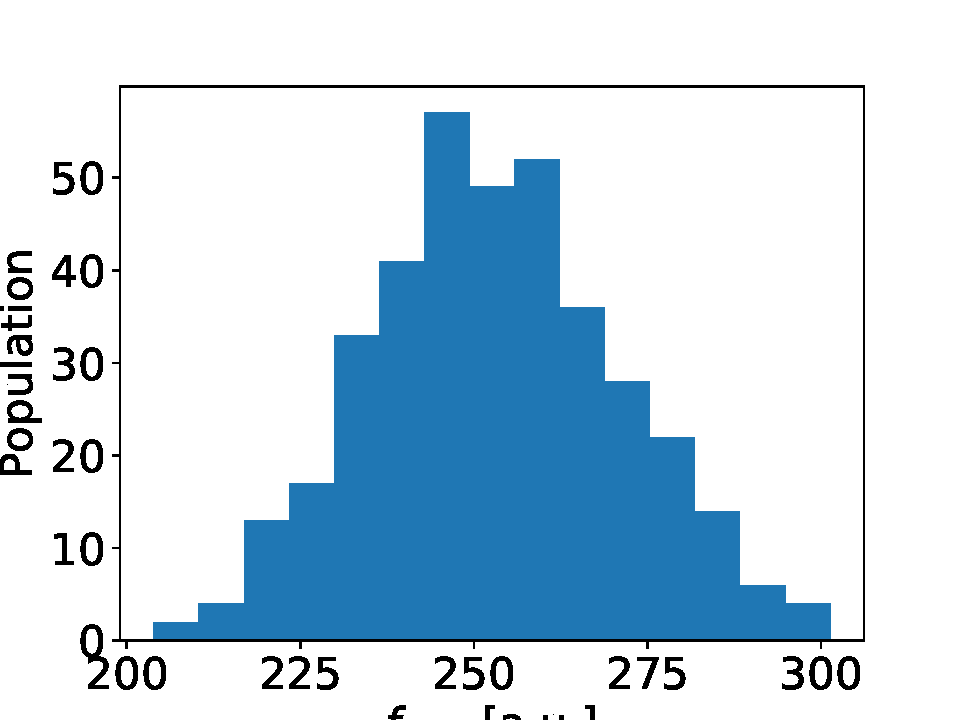
\includegraphics[width=8cm]{../../images/fig_max_hist/180518_ch02v050r0d3_int252_time10000_fig_max_hist.pdf}
% 	\label{fig:fig_max_hist/180518_ch02v050r0d3_int252_time10000_fig_max_hist.pdf}
% 	\caption{Histogram before normalization}
% \end{figure}

% \subsection{qq-plot}
% 次に、発振周波数のqqplotを描く。qqpoltとは得られたデータと理論分布を比較し、その類似度を調べるためのグラフである。横軸は分周期にかけられた

% \begin{figure}[H]
% 	\centering
% 	\includegraphics[width=8cm]{../../images/fig_max_qqplot/180518_ch02v050r0d3_int252_time10000_fig_max_qqplot.pdf}
% 	\label{fig:fig_max_qqplot/180518_ch02v050r0d3_int252_time10000_fig_max_qqplot.pdf}
% \end{figure}

\section{正規化後の結果}
\subsection{ヒストグラム}
まず、発振周波数のヒストグラムを描く。横軸は各分周器にかけられた発振周波数の各セクションでの最大値と最小値の差を最大値で割った値である。縦軸はその周波数を示した回数である。図\ref{fig:fig_delta_hist/180518_ch02v050r0d3_int252_time10000_fig_delta_hist.pdf}は$p=655, n=140$の時のヒストグラムである。

\begin{figure}[H]
	\centering
	\includegraphics[width=10cm]{../../images/fig_delta_hist/180518_ch02v050r0d3_int252_time10000_fig_delta_hist.pdf}
	\label{fig:fig_delta_hist/180518_ch02v050r0d3_int252_time10000_fig_delta_hist.pdf}
	\caption{Histogram of frequency after normalized}
\end{figure}

% \begin{figure}[H]
% 	\centering
% 	\subfigure[7段]{
% 		\includegraphics[width=5cm]{../../images/fig_delta_hist/180522_ch02v050r36d3_int247_time10000_fig_delta_hist.pdf}
% 		\label{fig:fig_delta_qqplot/180522_ch02v050r36d3_int247_time10000_fig_delta_qqplot.pdf}
% 	}
% 	\subfigure[13段]{
% 		\includegraphics[width=5cm]{../../images/fig_delta_hist/180522_ch02v050r41d3_int163_time10000_fig_delta_hist.pdf}
% 		\label{fig:fig_delta_qqplot/180522_ch02v050r41d3_int163_time10000_fig_delta_qqplot.pdf}
% 	}
% 	\subfigure[19段]{
% 		\includegraphics[width=5cm]{../../images/fig_delta_hist/180522_ch02v050r42d3_int114_time10000_fig_delta_hist.pdf}
% 		\label{fig:fig_delta_qqplot/180522_ch02v050r42d3_int114_time10000_fig_delta_qqplot.pdf}
% 	}
% 	\subfigure[29段]{
% 		\includegraphics[width=5cm]{../../images/fig_delta_hist/180522_ch02v050r43d3_int75_time10000_fig_delta_hist.pdf}
% 		\label{fig:fig_delta_qqplot/180522_ch02v050r43d3_int75_time10000_fig_delta_qqplot.pdf}
% 	}
% 	\subfigure[59段]{
% 		\includegraphics[width=5cm]{../../images/fig_delta_hist/180522_ch02v050r44d3_int41_time10000_fig_delta_hist.pdf}
% 		\label{fig:number_of_network_operations_comparison_5}
% 	}
% 	\caption{Number of network operations comparison}
% 	\label{fig:number_of_network_operations_comparison}
% \end{figure}

\subsection{qq-plot}
次に、発振周波数のqqplotを描く。qqpoltとは得られたデータと理論分布を比較し、その類似度を調べるためのグラフである。横軸は各分周器にかけられた発振周波数の各セクションでの最大値と最小値の差を最大値で割った値である。縦軸は理論分位数となっている。

\begin{figure}[H]
	\centering
	\subfigure[p=655]{
		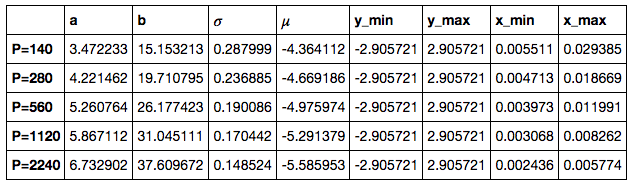
\includegraphics[width=10cm]{../../images/p655.pdf}
		\label{fig:p655}
	}
	\subfigure[n=420]{
		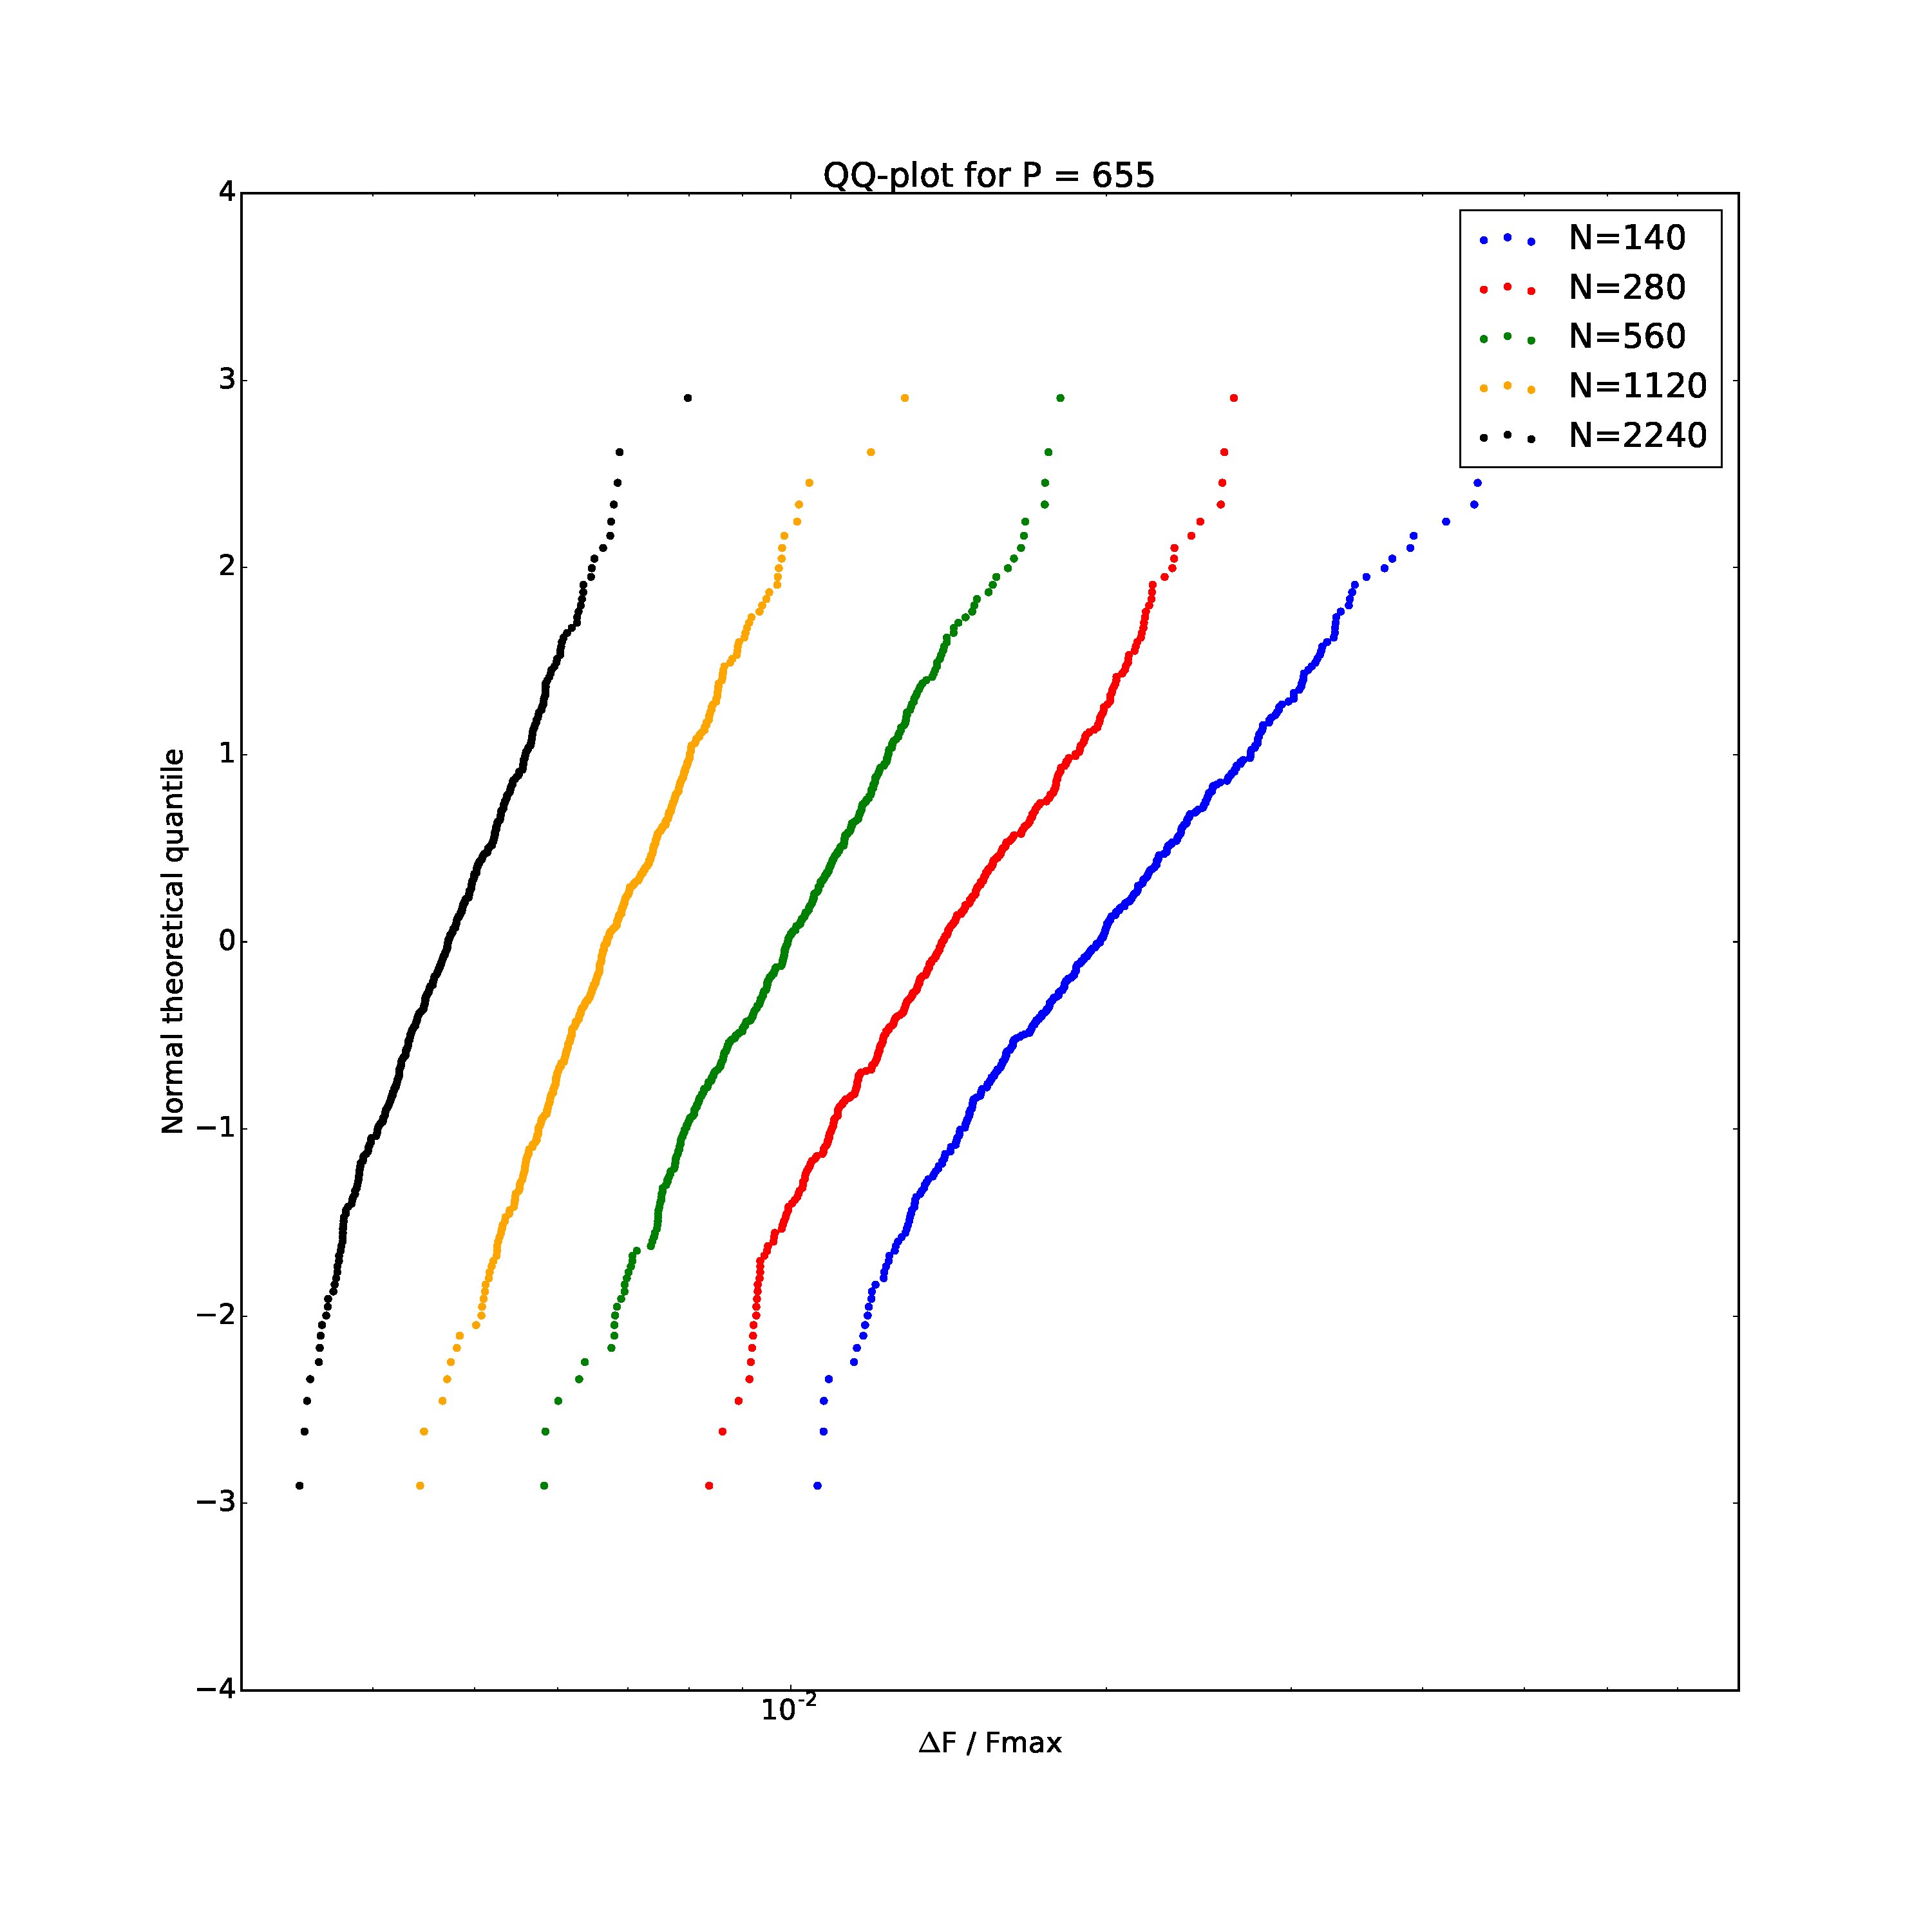
\includegraphics[width=10cm]{../../images/n420.pdf}
		\label{fig:n420}
	}
	\caption{the effect of the edge length of FET}
	\label{fig:the_effect_of_the_size_of_fet}
\end{figure}

図\ref{fig:the_effect_of_the_size_of_fet}はFETの1辺の長さを変化させた時の結果である。どのスロットの値も正規分布に従っていて、FETの面積が大きくなればなるほど$\Delta F / F_max$の値は小さくなることがわかる。

\begin{figure}[H]
	\centering
	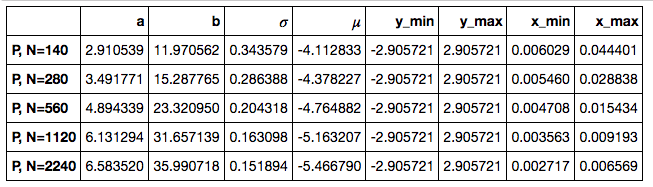
\includegraphics[width=10cm]{../../images/square.pdf}
	\label{fig:square}
	\caption{the effect of the area of FET}
\end{figure}

図\ref{fig:square}はFETの両辺の長さを変化させた時の結果である。1辺を変化させた時の結果と似ているが、FETの面積が小さい時に理論分布との類似度が下がっていると考察する。

\begin{figure}[H]
	\centering
	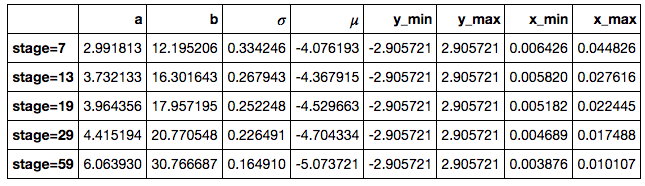
\includegraphics[width=10cm]{../../images/stage.pdf}
	\label{fig:stage}
	\caption{the effect of the number of stages}
\end{figure}

図\ref{fig:stage}はリングオシレーターの段数を変化させた時の結果である。段数が大きくなればなるほど$\Delta F / F_max$の値は小さくなることがわかる。また、それぞれのセクションにて$\Delta F / F_max$が大きいところで理論分布との類似度が下がっていると考察する。



\end{document}
